We kick off with the example
\begin{example} \label{ex:feedback filter}
    Consider the sequence $x[n] \in \R$, which represents the signal evolving in time. Let:
    \begin{equation*}
        y[0] = x[0], \quad y[n] = x[n] + \alpha y[n-1] \; \forall n > 0
    \end{equation*}

    The structure of the formula suggests, that we should use an induction to get a closed formula for $y$:

    \begin{enumerate}
        \item[Base.] $y[0] = x[0] = \alpha^0 x[0]$
        \item[Step.] Assume that it holds for some $n$, that
              \begin{equation}
                  y[n] = \sum_{j=0}^{n} \alpha^{n-j} x[j]
                  \label{eq:feedback filter closed form}
              \end{equation}
              Then:
              \[\begin{aligned}
                      y[n + 1]
                       & = x[n + 1] + \alpha y[n]
                      = \alpha^0 x[n + 1] + \alpha \sum_{j=0}^{n} \alpha^{n-j} x[j]
                      \\ & = \alpha^0 x[n + 1] + \sum_{j=0}^{n} \alpha^{n+1-j} x[j]
                      = \sum_{j=0}^{n + 1} \alpha^{n+1-j} x[j]
                  \end{aligned}\]
    \end{enumerate}

    Note that the formula \eqref{eq:feedback filter closed form} can be written as a following convolution:
    \[y[n]
        = \sum_{j=0}^{n} \alpha^{n-j} x[j]
        = \sum_{j=0}^{n} h_n[n-j] x[j]
        = x \ast h_n\]

    Thus:
    \[h_n = {\left(\alpha^0, \alpha^1, \dots, \alpha^{n}\right)}^{T}\]

    As in the case of Ideal low pass filter in Section~\ref{sec:ideal lpf} we got an impulse response of the filter introduced above. The only difference is that this filter has an impulse response with the size proportional to the sample size. That said the IR size grows infinitely in time unlike the IR of an ideal LPF, which has the same size for each frame.
\end{example}

\newpage
\subsection{Stability}
Let us consider the general form of the filters we would like to analyze:
\begin{equation}
    y[n] = \sum_{i=0}^{N} b_i x[n - i] + \sum_{i=1}^{M} a_i y[n - i] \label{eq:IIR def}
\end{equation}

\begin{theorem}[Discrete Tonelli] \label{thm:discrete tonelli}
    Let us have the sequence $x_{nk} \in [0;\infty]$. Then:
    \[
        \sum_{k=-\infty}^{\infty} \sum_{n=-\infty}^{\infty} x_{nk}
        = \sum_{n=-\infty}^{\infty} \sum_{k=-\infty}^{\infty} x_{nk}\]
\end{theorem}
\begin{proof}
    We have that the space $(\Z, \curlyP(\Z), \mu)$ is $\sigma$-finite with the counting measure $\mu$. This is easily verified using that $\Z = \bigcup_{k \in \Z} \{k\}$. Therefore the product measure $\mu \otimes \mu$ is well-defined and unique.

    Define
    \[
        f:\Z \times \Z \to [0;\infty], \quad (n, k) \mapsto x_{nk}\]

    We define the function slices as:
    \begin{align*}
        f_n: \Z \to [0;\infty]     & , \quad k \mapsto x_{nk} \\
        f^{(k)}: \Z \to [0;\infty] & , \quad n \mapsto x_{nk}
    \end{align*}

    And we observe that $\ind_{[-K, K]} \cdot f_{n} = \sum_{k=-K}^{K} \ind_{\{k\}} \cdot x_{nk} \uparrow f_n$, so using the the fact that each $\ind_{[-K, K]} \cdot f_{n}$ is simple:
    \[\int_{\Z} \ind_{[-K, K]} \cdot f_{n} \dx{\mu(k)}
        = \sum_{k=-K}^{K} \mu(\{k\}) x_{nk}
        = \sum_{k=-K}^{K} x_{nk} \]
    Using Monotone convergence theorem:
    \begin{align*}
        \sum_{k=-\infty}^{\infty} x_{nk}
         & = \lim_{K \to \infty} \int_{\Z} \ind_{[-K, K]} \cdot f_{n} \dx{\mu(k)}
        \\ &= \int_{\Z} \lim_{K \to \infty} \left( \ind_{[-K, K]} \cdot f_{n} \right) \dx{\mu(k)}
        = \int_{\Z} f_{n}(k) \dx{\mu(k)}
    \end{align*}

    Using the similar construction:
    \[g:\Z \to [0;\infty], \quad n \to \int_{\Z} f_{n}(k) \dx{\mu(k)}\]

    And its approximation:
    \[\ind_{[-N, N]} \cdot g
        = \sum_{n=-N}^{N} \left(\ind_{\{n\}}\int_{\Z} f_{n}(k) \dx{\mu(k)}\right) \uparrow g\]
    since the integral of the positive function $f_n$ is positive as well, so $g \geq 0$.
    \begin{align*}
        \sum_{n=-\infty}^{\infty} \sum_{k=-\infty}^{\infty} x_{nk}
         & = \lim_{N \to \infty} \int_{\Z} \ind_{[-N, N]} \cdot g(n) \dx{\mu(n)}
        \\ &= \int_{\Z} \lim_{N \to \infty} \left( \ind_{[-N, N]} \cdot g(n) \right) \dx{\mu(n)}
        \\ &= \int_{\Z} g(n) \dx{\mu(n)}
        = \int_{\Z} \int_{\Z} f_{n}(k) \dx{\mu(k)} \dx{\mu(n)}
    \end{align*}

    Using Tonelli's theorem we have:
    \[\int_{\Z \times \Z} f \dx{\mu \otimes \mu (n, k)}
        = \int_{\Z} \int_{\Z} f_{n}(k) \dx{\mu(k)} \dx{\mu(n)}
        = \int_{\Z} \int_{\Z} f^{(k)}(n) \dx{\mu(n)} \dx{\mu(k)}\]

    In a similar fashion we can show for the slice at a height $k$:
    \[\sum_{k=-\infty}^{\infty} \sum_{n=-\infty}^{\infty} x_{nk}
        = \int_{\Z} \int_{\Z} f^{(k)}(n) \dx{\mu(n)} \dx{\mu(k)}\]

    Which proves:
    \[\sum_{k=-\infty}^{\infty} \sum_{n=-\infty}^{\infty} x_{nk}
        = \int_{\Z \times \Z} f \dx{\mu \otimes \mu (n, k)}
        = \sum_{n=-\infty}^{\infty} \sum_{k=-\infty}^{\infty} x_{nk} \]
\end{proof}

\begin{theorem}[Discrete Fubini] \label{thm:discrete fubini}
    Let us have the sequence $z_{nk} \in \C$ with
    \[\sum_{(n, k) \in Z \times \Z} |z_{nk}| < \infty\]
    Then:
    \[
        \sum_{k=-\infty}^{\infty} \sum_{n=-\infty}^{\infty} z_{nk}
        = \sum_{n=-\infty}^{\infty} \sum_{k=-\infty}^{\infty} z_{nk}\]
\end{theorem}
\begin{proof}
    Let $x_{nk} \in \R$ and define:
    \[
        x_{nk}^+ = \begin{cases}
            x_{nk}, \; x_{nk} \geq 0 \\
            0, x_{nk} < 0
        \end{cases} \quad
        x_{nk}^- = \begin{cases}
            -x_{nk}, \; x_{nk} < 0 \\
            0, x_{nk} \geq 0
        \end{cases} \]

    Recall that if both sums $\sum_{n=-\infty}^{\infty} a_n$ and $\sum_{n=-\infty}^{\infty} b_n$ with $a_n, b_n \in \R$ exist then:
    \begin{align*}
        \sum_{n=-\infty}^{\infty} (a_n - b_n)
         & = \lim_{N\to \infty} \left(\sum_{n=-N}^{N} (a_n - b_n)\right)
        \\ &= \lim_{N\to \infty} \left(\sum_{n=-N}^{N} a_n - \sum_{n=-N}^{N} b_n\right)
        \\ &= \lim_{N\to \infty} \left(\sum_{n=-N}^{N} a_n\right) - \lim_{N\to \infty}  \left(\sum_{n=-N}^{N} b_n\right)
        \\ &= \sum_{n=-\infty}^{\infty} a_n - \sum_{n=-\infty}^{\infty} b_n
    \end{align*}

    We have that:
    \[
        \left|\sum_{k = -\infty}^{\infty} x^{\pm}_{nk} \right|
        = \sum_{k = -\infty}^{\infty} x^{\pm}_{nk}
        \leq \sum_{k=-\infty}^{\infty} |x_{nk}| \quad \forall k \in \Z < \infty\]
    so using the comparison principle we have the following:
    \[
        \sum_{n = -\infty}^{\infty} \sum_{k = -\infty}^{\infty} x^{\pm}_{nk} < \infty\]

    Therefore:
    \begin{align*}
        \sum_{n=-\infty}^{\infty} \sum_{k=-\infty}^{\infty} x_{nk}
        = \sum_{n=-\infty}^{\infty} \sum_{k=-\infty}^{\infty} (x^+_{nk} - x^-_{nk})
        = \sum_{n=-\infty}^{\infty} \sum_{k=-\infty}^{\infty} x^+_{nk} - \sum_{n=-\infty}^{\infty} \sum_{k=-\infty}^{\infty} x^-_{nk}
    \end{align*}

    The sum order can be interchanged by Theorem~\ref{thm:discrete tonelli}:
    \begin{align*}
        \sum_{n=-\infty}^{\infty} \sum_{k=-\infty}^{\infty} x^+_{nk} - \sum_{n=-\infty}^{\infty} \sum_{k=-\infty}^{\infty} x^-_{nk}
         & = \sum_{k=-\infty}^{\infty} \sum_{n=-\infty}^{\infty} x^+_{nk} - \sum_{k=-\infty}^{\infty} \sum_{n=-\infty}^{\infty} x^-_{nk}
        \\ &= \sum_{k=-\infty}^{\infty} \sum_{n=-\infty}^{\infty} (x^+_{nk} - x^-_{nk})
        \\ &= \sum_{k=-\infty}^{\infty} \sum_{n=-\infty}^{\infty} x_{nk}
    \end{align*}

    This argument can be generalized for $z_{nk} \in C$ using the auxiliary sequences $r_{nk} = \real(z_{nk})$ and $s_{nk} = \imag(z_{nk})$. Both are absolutely summable since $|r_{nk}|, |s_{nk}| < |z_{nk}|$. This immediately results in the desired result applying the previous argumentation to $r_{nk}$ and $s_{nk}$.
\end{proof}

\begin{lemma}[Z-transform properties]
    Let $x \ztransform X(z)$ and $y \ztransform Y(z)$. The following holds:
    \begin{enumerate}[label=\thelemma.\arabic*]
        \item \label{lm:z time shift} $x[n-k] \ztransform z^{-k}X(z)$
        \item \label{lm:z linearity} $\alpha x[n] + \beta y[n] \ztransform \alpha X(z) + \beta Y(z)$
        \item \label{lm:z reverse} $x[-n] \ztransform \alpha X(z^{-1})$
    \end{enumerate}
\end{lemma}
\begin{proof} \hfill
    \begin{enumerate}
        \item
              \begin{align*}
                  \sum_{n=-\infty}^{\infty} x[n-k] z^{-n}
                   & = \sum_{m=-\infty}^{\infty} x[m] z^{-(m+k)}
                  \\ &= z^{-k} \sum_{m=-\infty}^{\infty} x[m] z^{-m}
                  \\ &= z^{-k} X(z)
              \end{align*}
        \item We assume that both $X(z)$ and $Y(z)$ converge for the given value of $z$
              \begin{align*}
                  \sum_{n=-\infty}^{\infty} (\alpha x[n] + \beta y[n])z^{-n}
                   & = \sum_{n=-\infty}^{\infty} \alpha x[n] z^{-n} + \beta y[n] z^{-n}
                  \\ &= \alpha \sum_{n=-\infty}^{\infty} x[n] z^{-n} + \beta \sum_{n=-\infty}^{\infty} y[n] z^{-n}
                  \\ &= \alpha X(z) + \beta Y(z)
              \end{align*}
        \item
              \[\sum_{n=-\infty}^{\infty} x[-n] z^{-n}
                  \underset{k = -n}{=} \sum_{k=-\infty}^{\infty} x[k] z^{k}
                  = \sum_{k=-\infty}^{\infty} x[n] {\left(z^{-1}\right)}^{-k}
                  = X(z^{-1})\]
    \end{enumerate}
\end{proof}

Taking the Z-transform of \eqref{eq:IIR def}:
\[
    y[n] \ztransform \sum_{i=0}^{N} b_i z^{-i} X(z) + \sum_{i=1}^{M} a_i z^{-i} Y(z)\]

That is:
\[Y(z) = \sum_{i=0}^{N} b_i z^{-i} X(z) + \sum_{i=1}^{M} a_i z^{-i} Y(z)\]
\[Y(z) - \sum_{i=1}^{M} a_i z^{-i} Y(z) = \sum_{i=0}^{N} b_i z^{-i} X(z)\]
\begin{equation}
    \frac{Y(z)}{X(z)} = \frac{\sum_{i=0}^{N} b_i z^{-i}}{1 - \sum_{i=1}^{M} a_i z^{-i}}
    \label{eq:transfer func}
\end{equation}

This is called a transfer function and it is crucial for analyzing the filter's behaviour. Recall the definition of \ref{eq:DFT}:
\[z_k
    = \frac{1}{\sqrt{N}}\sum_{k =0}^{N-1} \omega_N^{-kj} y_k
    = \frac{1}{\sqrt{N}}\sum_{k =0}^{N-1} {\left(e^{\frac{2\pi i j}{N}}\right)}^{-k} y_k\]

Now we denote $z = e^{\frac{2\pi i j}{N}}$ and drop the normalization factor in front. The expression becomes:
\[\sum_{k =0}^{N-1} z^{-k} y_k\]
is exactly the Z-transform of the signal $y$ (embedded into the infinite sequence). In general as $N$ gets large we may assume that for any $\omega \in [0, 2\pi]$ exists $j\in \N$ such that $\frac{2\pi j}{N} \approx \omega$, which allows us to compute the presence of any frequency in the range $[0, 2\pi]$ by evaluating the signal Z-transform at a point $z = e^{i\omega}$. Moreover the Theorem~\ref{thm:discrete convolution theorem} suggests that the function $H(z)$ represents an impulse response as it essentially does deconvolution in the frequency (z) domain.

\begin{lemma}[Partial fraction expansion] \label{lm:partial fraction}
    Let $P(x) \in \C_M[x]$, $a_i \in \C$ for $i \in \{1, \dots, N\}$ and $M<N$
    \[Q(x) = \frac{P(x)}{\prod_{k=1}^{N} (1-a_kx)}\]
    with $a_i \neq a_j \;\forall i\neq j$ and $a_i \neq 0$.

    Then the function $Q(x)$ can be expressed in the following form:
    \[Q(x) = \sum_{i=1}^{N} \frac{A_i}{(1-a_i x)}\]
    and moreover this representation is unique.
\end{lemma}
\begin{proof}
    Let $Q_i(x) = \prod_{k\neq i}^{N} (1-a_kx)$. Consider their linear combination:
    \[\sum_{i=1}^{N} \lambda_i Q_i(x) = 0\]
    Substitute $a_j^{-1}$, which is well defined since $a_j \neq 0 \; \forall j\in \N$. We observe that $Q_i(a_j^{-1}) = 0$ for $i\neq j$ since $Q_i$ contains the term $(1-a_jx)$. Also $a_ia_j^{-1} \neq 1 \; \forall i\neq j$ since $a_i \neq a_j$, so $Q_j(a_j^{-1}) \neq 0$. Then:
    \[\sum_{i=1}^{N} \lambda_i Q_i(a_j^{-1}) = \lambda_j Q_j(a_j^{-1}) = 0\]

    Since the field $(\C, +, \cdot)$ is zero divisor free we must have $\lambda_j = 0$. This holds for all $j\in \{1, \dots, N\}$.

    Thus $Q_i$'s form the basis of $\C_{N-1}[x]$ as $\dim \C_{N-1}[x] = N$, hence in particular we can decompose every polynomial in $\C_{M}[x]$ using the linear combination of $Q_i$:
    \begin{align*}
        \frac{P(x)}{\prod_{k=1}^{N} (1-a_kx)}
        = \frac{\sum_{i=1}^{N} A_i Q_i}{\prod_{k=1}^{N} (1-a_kx)}
        = \sum_{i=1}^{N} \frac{A_i Q_i}{\prod_{k=1}^{N} (1-a_kx)}
        = \sum_{i=1}^{N} \frac{A_i}{1-a_ix}
    \end{align*}
    Thus we proved the existence of partial fraction decomposition whenever the numerator degree is less than the degree of denominator and denominator does not contain zero roots. Uniqueness follows from the basis properties.
\end{proof}

\begin{lemma}[Long division] \label{lm:long div}
    Let $P \in C_N[x]$ and $Q \in C_M[x]$ with $N \geq M > 0$ and $\deg P = N$, $\deg Q = M$. Then there exists a polynomial $q \in C_{N-M}[x]$ and $r \in C_{M-1}[x]$, s.t. $P = q\cdot Q + r$
\end{lemma}
\begin{proof}
    Let $P(x) = a_{N}x^N + \dots + a_1x + a_0$ and $Q(x) = b_{M}x^M + \dots + b_1x + b_0$ with $a_N \neq 0$ and $b_M \neq 0$ to ensure that polynomials have the proper degree.
    We prove this statement by induction:
    \begin{enumerate}
        \item[Base:] Let $N = M$. Set $q(x) = a_N / b_M$ and $r(x) = P(x) - q(x)\cdot Q(x)$.T his fraction is well defined since $b_M \neq 0$. $P = q\cdot Q + r$ follows by construction, so we need to show that $\deg r(x) \leq M$:
              \begin{align*}
                  r(x) = a_{N}x^N + \dots + a_1x + a_0 - \frac{a_N}{b_M} (b_{M}x^M + \dots + b_1x + b_0)
                   & =                 \\ a_{N}x^N + \dots + a_1x + a_0 - a_N x^M - \frac{a_N b_{M -1}}{b_M}x^{M-1} - \dots - \frac{a_N b_0}{b_M}
                   & \underset{N=M}{=} \\ a_{N}x^N + \dots + a_1x + a_0 - a_N x^N - \frac{a_N b_{N -1}}{b_N}x^{N-1} - \dots - \frac{a_N b_0}{b_N}
                   & =                 \\ a_{M-1}x^{M-1} + \dots + a_1x + a_0 - \frac{a_M b_{M -1}}{b_N}x^{M-1} - \dots - \frac{a_M b_0}{b_M}
              \end{align*}

              That is $\deg r \leq M-1$
        \item[Step:] Suppose the statement holds for some $N > M$. Then:
              \begin{align*}
                  P(x)
                   & = a_{N+1}x^{N+1} + \dots + a_1x + a_0
                  = x(a_{N+1}x^{N} + \dots + a_2x + a_1) + a_0
                  \\ &\underset{(a)}{=} x (q(x)\cdot Q(x) + r(x)) + a_0
                  = (xq(x)) \cdot Q(x) + (xr(x) + a_0)
              \end{align*}
              where (a) follows from the induction hypothesis, therefore $\deg q \leq N-M$ and $\deg r \leq M - 1$.

              Note that $\deg xq \leq N+1-M$ and $\deg xr \leq M,\; \deg a_0 = 0$. If the degree of $xr(x) + a_0$ is exactly $M$ we may use the base case to find the decomposition $xr(x) = \tilde{q}(x)Q(x) + \tilde{r}(x)$ where $\deg \tilde{q} = 0$ and $\deg \tilde{r} \leq M-1$. Then $q^*(x) = xq(x) + \tilde{q}(x),\; \deg q^* \leq N+1-M$ and $P(x) = q^*(x)Q(x) + \tilde{r}(x)$
    \end{enumerate}
\end{proof}

\begin{theorem} \label{thm:stability}
    Let $X(z)$ be a $z$-tranform of a causal system $x[n]$ (i.e. $x[n] = 0, \; \forall n<0$). Moreover assume that $X$ is the rational function with distinct non-zero poles. Then $x[n]$ is absolutely summable if the pole with the maximum magnitude lies inside the unit circle.
\end{theorem}
\begin{proof}
    \[X(z) = \frac{P(z^{-1})}{Q(z^{-1})}\]
    If $\deg P = N \geq M = \deg Q$, then the Lemma~\ref{lm:long div} ensures that exist $q(z^{-1}), r(z^{-1})$ with $\deg q \leq N-M$ and $\deg r \leq M-1$, s.t. $P(z^{-1}) = q(z^{-1})Q(z^{-1}) + r(z^{-1})$. If $N < M$, then $q = 0$ and $r = P$
    \[X(z)
        = \frac{q(z^{-1})Q(z^{-1}) + r(z^{-1})}{Q(z^{-1})}
        = q(z^{-1}) + \frac{r(z^{-1})}{Q(z^{-1})}\]

    Let $d_1, \dots, d_M$ be the poles of $X$ (distinct and non-zero by assumption), so $Q(z^{-1}) = \prod_{i=1}^{M} (1 - d_iz^{-1})$

    Using the Lemma~\ref{lm:partial fraction} we have that exist $A_1, \dots, A_M$, such that:
    \[\frac{r(z^{-1})}{Q(z^{-1})}
        = \sum_{i=1}^{M} \frac{A_i}{1 - d_iz^{-1}}\]
    \[X(z)
        = q(z^{-1}) + \sum_{i=1}^{M} \frac{A_i}{1 - d_iz^{-1}}
        = \sum_{i = 0}^{N-M} c_i z^{-i} + \sum_{i=1}^{M} \frac{A_i}{1 - d_iz^{-1}}\]

    The assumption about causality allows us to uniquelly determine the inverse z-transform by inspecting \href{https://en.wikipedia.org/wiki/Z-transform#Table_of_common_Z-transform_pairs}{the table}.
    \[c_i z^{-i} \iztransform c_i\delta[n-i]\]
    \[\frac{A_i}{1 - d_iz^{-1}} \iztransform A_i d_i^n u[n]\]

    Using the Lemma~\ref{lm:z linearity}:
    \[\sum_{i = 0}^{N-M} c_i z^{-i} + \sum_{i=1}^{M} \frac{A_i}{1 - d_iz^{-1}} \iztransform
        \sum_{i = 0}^{N-M} c_i\delta[n-i] + \sum_{i=1}^{M} A_i d_i^n u[n]\]
    \[\sum_{n=0}^{\infty} |x[n]|
        = \sum_{n=-\infty}^{\infty} \left|\sum_{i = 0}^{N-M} c_i\delta[n-i] + \sum_{i=1}^{M} A_i d_i^n u[n] \right|\]

    Note that $\delta[n-i] = 1$ if and only if $n = i$ and zero elsewhere.
    \begin{align*}
        \sum_{n=-\infty}^{\infty} |x[n]| & \leq
        \sum_{n=-\infty}^{\infty} \sum_{i = 0}^{N-M} |c_i\delta[n-i]| + \sum_{n=-\infty}^{\infty} \sum_{i=1}^{M} |A_i d_i^n u[n] |
        \\ &= \sum_{i = 0}^{N-M} |c_i| + \sum_{n=-\infty}^{\infty} \sum_{i=1}^{M} |A_i d_i^n u[n]|
    \end{align*}

    By Theorem~\ref{thm:discrete tonelli} and the proper extention of the finite sum to the infinite one (with zeros wherever the sequence is not defined):
    \[\sum_{i = 0}^{N-M} |c_i| + \sum_{n=-\infty}^{\infty} \sum_{i=1}^{M} |A_i d_i^n u[n]|
        = \sum_{i = 0}^{N-M} |c_i| +  \sum_{i=1}^{M} \sum_{n=-\infty}^{\infty} |A_i d_i^n u[n]|\]

    And one can note that it converges if and only if
    \[\sum_{n=-\infty}^{\infty} |A_i d_i^n u[n]|
        = |A_i| \sum_{n=0}^{\infty} |d_i^n| < \infty
        \quad \forall i \in \{1, \dots, M\}\]
    This is the sum of geometric series, hence converges if and only if $|d_i|<1$. We need this to hold for all $i\in \{1, \dots, M\}$, so $\max_{i} |d_i| < 1$
\end{proof}
\begin{theorem} \label{thm:convolution theorem z transform}
    Let $x \ztransform X(z)$ and $y \ztransform Y(z)$, with both $x,y$ being absolutely summable. Then $x \ast y \ztransform X(z)\cdot Y(z)$
\end{theorem}
\begin{proof}
    \[
        h[n] = x \ast y
        = \sum_{k=-\infty}^{\infty} x[k] y[n-k]\]
    By Theorem~\ref{thm:discrete tonelli}:
    \begin{align*}
        \sum_{n=-\infty}^{\infty} |h[n]|
         & = \sum_{n=-\infty}^{\infty} \sum_{k=-\infty}^{\infty} |x[k] y[n-k]|
        \\ &\leq \sum_{k=-\infty}^{\infty} \left( |x[k]| \sum_{n=-\infty}^{\infty} |y[n-k]| \right)
        \\ &= \sum_{n=-\infty}^{\infty} |y[n]| \cdot \sum_{k=-\infty}^{\infty} |x[k]| < \infty
    \end{align*}

    By applying Theorem~\ref{thm:discrete fubini} and Lemma~\ref{lm:z time shift} (time shift property):
    \begin{align*}
        \sum_{n=-\infty}^{\infty} h[n] z^{-n}
         & = \sum_{n=-\infty}^{\infty} \sum_{k=-\infty}^{\infty} x[k] y[n-k] z^{-n}
        \\ &= \sum_{k=-\infty}^{\infty} x[k] \sum_{n=-\infty}^{\infty} y[n-k] z^{-n}
        \\ &= Y(z) \sum_{k=-\infty}^{\infty} x[k] z^{-k}
        \\ &= X(z) Y(z)
    \end{align*}
\end{proof}

We say that z-transform converges if the series
\[\sum_{n=-\infty}^{\infty} |x[n]z^{-n}| = \sum_{n=-\infty}^{\infty} |x[n]|r^{-n}\]
converges\footnote{eq. (3.7)~\cite{oppenheim2010discrete}}. It can be easily seen that if the z transform converges for some point located at the distance $r$ to the origin, then it converges for any point at the circle with radius $r$ centered at the origin. This immediately yields the following equivalence:
\[X(e^{i\omega})\;\text{converges}\; \forall \omega \in [0, 2\pi] \Leftrightarrow x[n]\;\text{absolutely summable}\]

Return to the Example~\ref{ex:feedback filter}:
\[y[n] = x_n + \alpha y[n-1]\]

Its transfer function is:
\[H(z) = \frac{1}{1 - \alpha z^{-1}}\]
which has the only pole at $z = \alpha$, for which we require $|\alpha|< 1$, so that the ROC of $H$ includes the unit circle.

By definition of the tranfer function:
\[Y(z) = X(z)H(z)\]

Let $X \iztransform y$ and $H \iztransform h$, where both $x$ and $h$ are right-sided sequences.

Consider $(x \ast h)[n] = \sum_{k = -\infty}^{\infty} x[k] h[n-k] = 0$. For $n<0$ we have that $n - k \geq 0 \Leftrightarrow k \leq n < 0$. In this case we have that $x[k] = 0$ since $k < 0$, so $(x \ast h)[n] = 0$.

By Theorem~\ref{thm:convolution theorem z transform} we have that $X(z)H(z) \iztransform x \ast h := y$ as we require $y$ to be right-sided, so the inverse z transform is unique. If all the poles of the tranfer function lie inside of the unit circle, then by Theorem~\ref{thm:stability} we have that $h$ is absolutely summable. Moreover the Theorem~\ref{thm:convolution theorem z transform} shows that the convolution of two absolutely summable sequences is absolutely summable as well. Therefore $y$ is absolutely summable and hence the filter is stable.

\begin{remark}[Sliding window average]
    Firstly we define the moving average of $N$ points:
    \[
        y[n]
        = \frac{1}{N} \sum_{k=n - N + 1}^{n} x[k]\]

    With the substitution $m = n - k$:
    \[
        \frac{1}{N} \sum_{k = n - N + 1}^{n} x[k]
        = \frac{1}{N} \sum_{m = 0}^{N-1} x[n-m]
        = \sum_{m = 0}^{N-1} h[m] x[n-m]
        = (x \ast h)[n]\]
    so we define a kernel:
    \[h[n] = \begin{cases}
            \frac{1}{N}, \; 0 \leq n < N, \\
            0, \; \text{otherwise}
        \end{cases}\]

    We compute the transfer fucntion:
    \[h[n]
        \ztransform \sum_{k = -\infty}^{\infty} h[k] z^{-k}
        = \frac{1}{N} \sum_{k = 0}^{N-1} z^{-k}
        = \frac{1}{N} \frac{1-z^{-N}}{1-z^{-1}}\]
    which as \eqref{eq:transfer func} suggests correponds to the following direct form:
    \[y[n] = y[n-1] + \frac{1}{N} (x[n] - x[n-N])\]

    Let us now plug in the definition of $y$:
    \begin{align*}
        y[n-1] + \frac{1}{N} (x[n] - x[n-N])
         & = \frac{1}{N} \left(\sum_{k = n - N}^{n - 1} x[k] + x[n] - x[n-N]\right)
        \\ &= \frac{1}{N} \sum_{k = n - N + 1}^{n} x[k]
        = y[n]
    \end{align*}

    This is exactly the idea behind prefix sums (in particular using prefix sums to compute sliding window average).
\end{remark}

\newpage
\subsection{Notch filter}
We want to construct the transfer function with the zeros corresponding to the frequency $\omega$. Its numerator then is the function $(z^{-1} - e^{i\omega})(z^{-1} - e^{-i\omega})$ since we need to cancel both positive and negative frequency oscillations. If we define the transfer function as is the frequency response looks as in the Figure~{fig:notch unscaled freq response}

\begin{figure}[htbp]
    \centering
    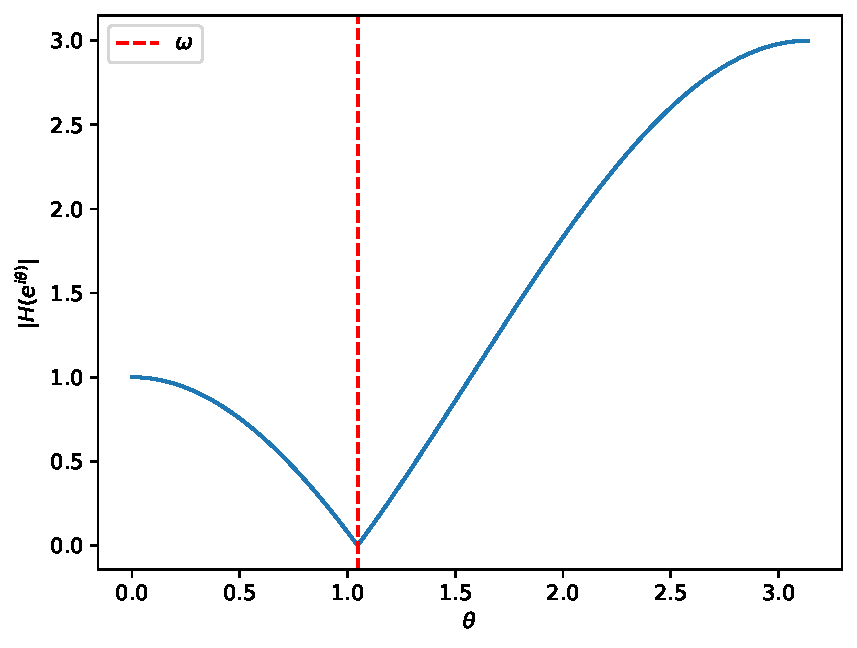
\includegraphics[width = 0.5\linewidth]{../plots/notch_freq_response_unscaled.pdf}
    \caption{The frequency response of $(z^{-1} - e^{i\omega})(z^{-1} - e^{-i\omega})$}
    \label{fig:notch unscaled freq response}
\end{figure}

As we can see from the Figure~\ref{fig:notch unscaled freq response} this filter produces a significant uneveness in the spectrum. Moreover we cannot really control the steepness of the constructed filter. To mitigate this we divide the transfer function we got previously by $(rz^{-1} - e^{i\omega})(rz^{-1} - e^{-i\omega})$. This helps to flatten the filter since $rz^{-1} - e^{i\omega} \approx (z^{-1} - e^{i\omega})$ for $r$ reasonably close to 1. Note that dividing the transfer function by this expression adds two poles at $d_1 = re^{-i\omega}$ and $d_2 = re^{i\omega}$, so for the filter to be stable (converge for the unit circle) the radius $r$ must be less that 1 by the Theorem~\ref{thm:stability}. The bigger the value of $r$, the closer the pole is to the zeros, so it makes the filter steeper as it "lifts" the surface around it.

Define:
\begin{align*}
    H(z)
    = \frac{(z^{-1} - e^{i\omega})(z^{-1} - e^{-i\omega})}{(rz^{-1} - e^{i\omega})(rz^{-1} - e^{-i\omega})}
     & = \frac{z^{-2} - (e^{-i\omega} + e^{i\omega})z^{-1} + 1}{r^2z^{-2} - r(e^{-i\omega} + e^{i\omega})z^{-1} + 1}
    \\ &= \frac{z^{-2} - 2\cos(\omega) z^{-1} + 1}{r^2z^{-2} - 2r\cos(\omega) z^{-1} + 1}
\end{align*}

\begin{figure}[ht!]
    \begin{minipage}{0.49\textwidth}
        \centering
        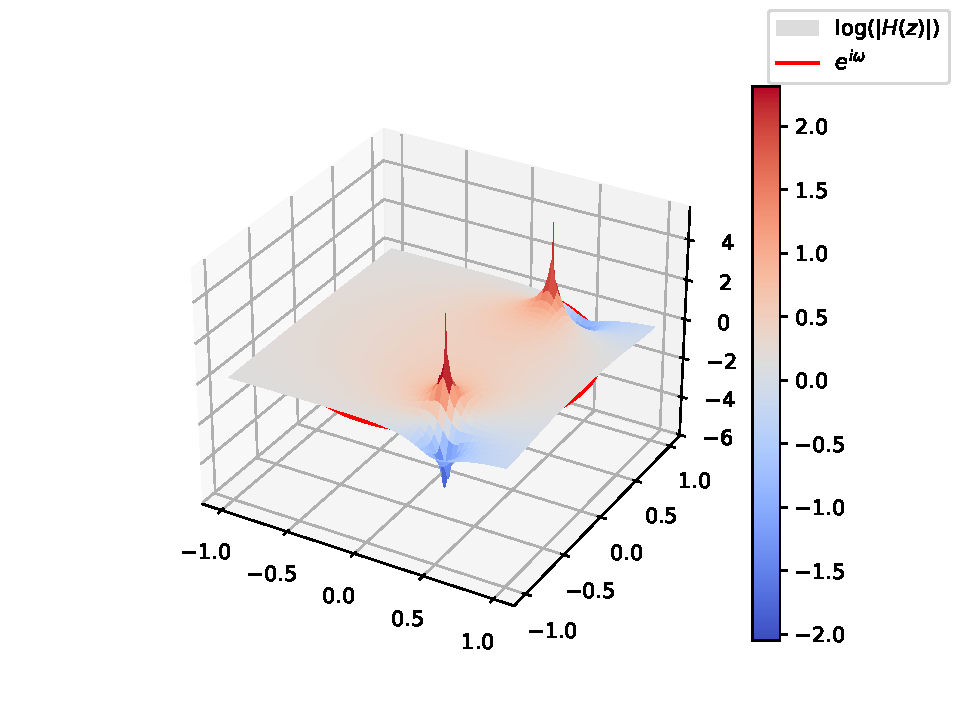
\includegraphics[width = \linewidth]{../plots/notch_topology.pdf}
        \caption{Notch filter topology}
        \label{fig:notch topology}
    \end{minipage}
    \begin{minipage}{0.49\textwidth}
        \centering
        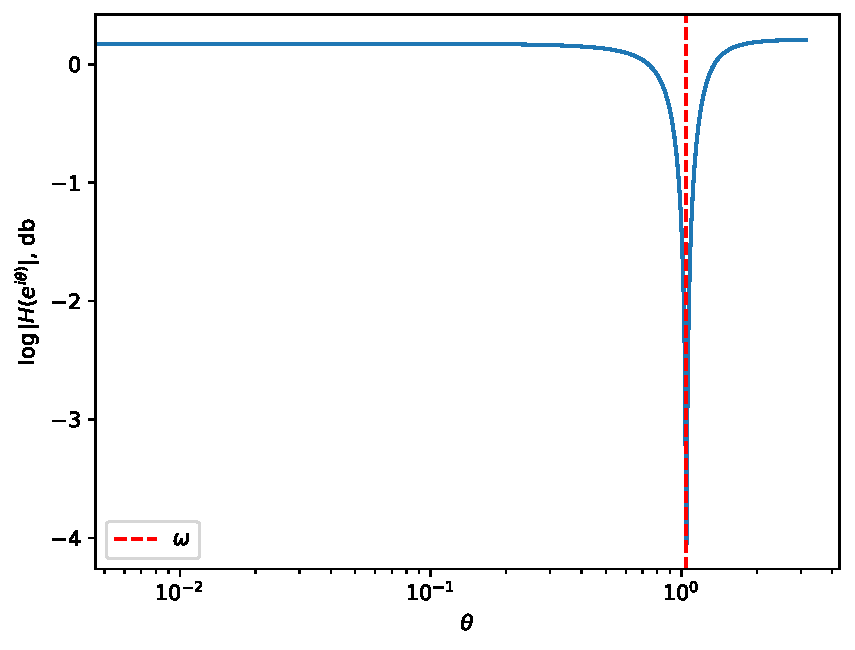
\includegraphics[width = \linewidth]{../plots/notch_freq_response.pdf}
        \caption{Notch filter frequency response}
        \label{fig:notch frequency response}
    \end{minipage}
\end{figure}

Note that there are two spike slightly inside of the red circle and two dips. Those are the poles and the zeros of $H$.

And its frequency response looks as in the Figure~\ref{fig:notch frequency response}

Note that for the transfer function $H(z)$ we have:
\[
    \overline{H(z)}
    =\overline{\frac{z^{-2} - 2\cos(\omega) z^{-1} + 1}{r^2z^{-2} - 2r\cos(\omega) z^{-1} + 1}}
    =\frac{\overline{z^{-2}} - 2\cos(\omega) \overline{z^{-1}} + 1}{r^2\overline{z^{-2}} - 2r\cos(\omega) \overline{z^{-1}} + 1}
    =H(\overline{z})\]

That means for the frequency $e^{-i\theta}$ the frequency response has the same magnitude as for $e^{i\theta}$, but inverted phase. By the Remark~\ref{ex:phase shift}, we have that the phase of the frequency response directly relates to the corresponding oscillation phase. This allows us the visualize also the phase response of the constructed filter (Figure~\ref{fig:notch phase response})
\begin{figure}[ht!]
    \begin{center}
        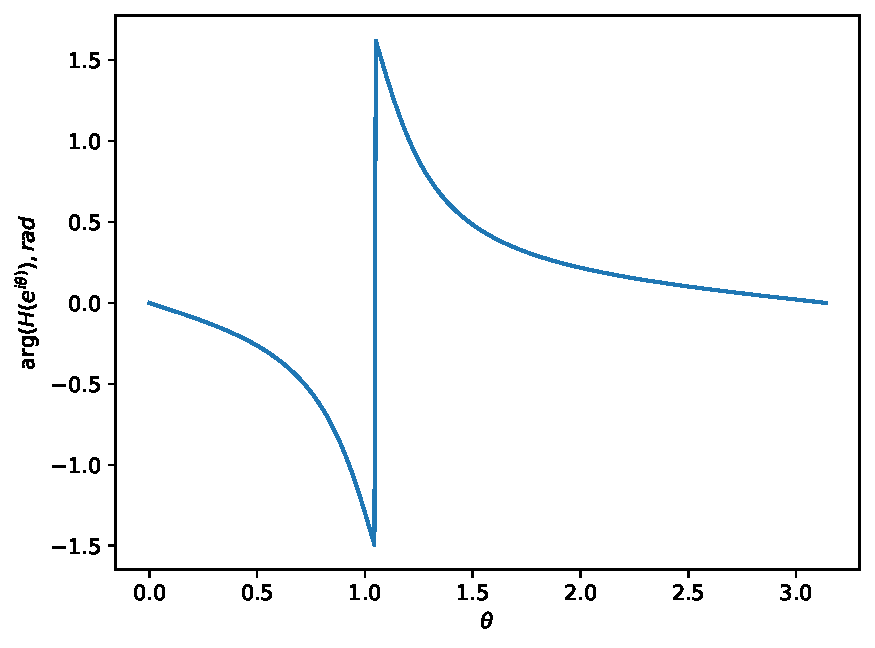
\includegraphics[width = 0.5\linewidth]{../plots/notch_phase_response.pdf}
    \end{center}
    \caption{The notch filter phase response}
    \label{fig:notch phase response}
\end{figure}

In a similar fashion we can build a peak filter by moving the zero of the filter closer to the origin, so that the pole influences the unit circle (frequnecy response) than the zeros do.
\begin{align*}
    H(z) = \frac{r_1^2 z^{-2} - 2 r_1 \cos(\omega) z^{-1} + 1}{r_2^2z^{-2} - 2 r_2 \cos(\omega) z^{-1} + 1}
    \qquad r_1 < r_2 < 1
\end{align*}

The notch filter then is the special case, where $r_1 = 1$.